\section{Results and Discussion}
\label{sec:results-and-discussion}

\subsection{Burnout Scores and Survey Associations}

The mean primary BAT-S score was 3.125 (SD 0.795), and the mean secondary score was 3.150 (SD 0.765). Seventeen of the 97 students (17.5\%) met the High criterion of a primary score of at least 4. Cronbach's alpha was 0.900 for the 12 items in the primary score and 0.944 for the 23 core items. Alpha measures how consistently the items in each set vary together.

Among the 11 questions tested, avoidance or procrastination had the largest Spearman correlation with the primary burnout score (\(\rho=0.445\)). Perceived workload and academic stress had correlations of 0.388 and 0.367, respectively. Of the three GenAI questions in the eight-input set, AI dependence had the largest correlation (0.377), followed by reliance on AI in place of independent thinking (0.331) and frequency of use (0.220). These exploratory estimates describe the association between each question and the burnout score, without adjustment for other questions or for multiple testing.

\subsection{Numerical Score Prediction}

The ridge regression comparison evaluated the five- and eight-input sets on the same held-out students. Adding the three GenAI questions reduced mean absolute error (MAE) for the primary score by 0.0300 points, from 0.6183 to 0.5883. For the secondary score, MAE decreased from 0.6001 to 0.5528 points. With the same eight inputs, XGBoost produced higher errors than ridge for both the primary score (0.6155 points) and the secondary score (0.5749 points).

In the matched ridge comparison of the 13- and 23-input sets, adding the GenAI questions reduced MAE from 0.6145 to 0.5933 points for the primary score and from 0.5874 to 0.5578 points for the secondary score. MAE decreased in all five repetitions for both scores. The training-mean and training-median benchmarks had primary-score MAEs of 0.6291 and 0.6262 points, respectively.

Table~\ref{tab:score-prediction-results} compares the primary-score errors for the full sample and the High group. Ordinary ridge with eight inputs tended to underestimate scores in the High group. With the same inputs, weighted ridge reduced High-group MAE from 0.9329 to 0.6649 points and increased overall MAE from 0.5883 to 0.6282 points.

The fixed blend gave equal weight to ridge and support vector regression (SVR). It achieved lower MAE than either component for the full sample and for the High group. Its overall MAE was higher than that of ordinary ridge with eight inputs. Selecting the blend weights in the inner folds increased both errors relative to the fixed blend.

\begin{table}[t]
\caption{Recorded Mean Absolute Error for the Primary Burnout Score}
\label{tab:score-prediction-results}
\centering
\footnotesize
\begin{tabular}{@{}lrr@{}}
\hline
Score procedure & Overall (points) & High (points) \\
\hline
Ordinary ridge, 5 inputs & 0.6183 & 1.0842 \\
Ordinary ridge, 8 inputs & 0.5883 & 0.9329 \\
Ordinary ridge, 13 inputs & 0.6145 & 1.0237 \\
Ordinary ridge, 23 inputs & 0.5933 & 0.9281 \\
Weighted ridge, 8 inputs & 0.6282 & 0.6649 \\
High-priority SVR, 23 inputs & 0.6282 & 0.6705 \\
Fixed ridge/SVR blend & 0.6160 & 0.6422 \\
Inner-selected blend & 0.6343 & 0.6664 \\
\hline
\end{tabular}
\end{table}

\subsection{High-Symptom Warning Performance}

Across five cross-validation repetitions, workload-only logistic regression detected an average of 16.0 of the 17 High students (94.1\% recall), and the eight-question forest detected 14.8 (87.1\% recall). Both averaged 28 false warnings among the 80 Below-high students (Fig.~\ref{fig:warning-counts}). Precision was 36.4\% for workload alone and 34.7\% for the forest.

\begin{figure}[t]
\centering
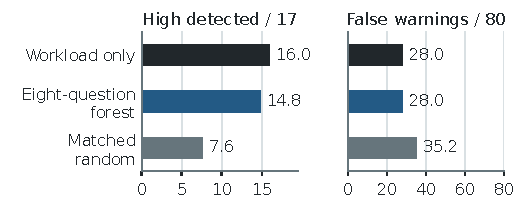
\includegraphics[width=\columnwidth]{figures/warning-counts.pdf}
\caption{Mean detections and false warnings per repetition on held-out students. The random reference shows expected counts when matched to the forest's number of warnings in each test fold.}
\label{fig:warning-counts}
\end{figure}

At the selected thresholds, workload-only logistic regression achieved higher balanced accuracy (79.6\% versus 76.0\%) and a higher \(F_2\) score (0.714 versus 0.668) than the selected forest. Across warning thresholds, the forest achieved higher average precision (0.527 versus 0.423), and workload-only logistic regression achieved a higher area under the receiver operating characteristic (ROC) curve (0.824 versus 0.809).

With training augmentation available during tuning, the forest detected an average of 0.4 more High students and issued 1.6 fewer false warnings than the forest tuned without augmentation.

The permutation test evaluated the selected forest against chance within the study sample (Fig.~\ref{fig:permutation-accuracy}). With the original labels, the forest achieved 76.0\% balanced accuracy. Across the 199 shuffled-label evaluations, mean balanced accuracy was 49.6\% and the maximum was 63.6\%. All shuffled-label results fell below the observed value, yielding a corrected one-sided permutation \(p\)-value of 0.005.

\begin{figure}[t]
\centering
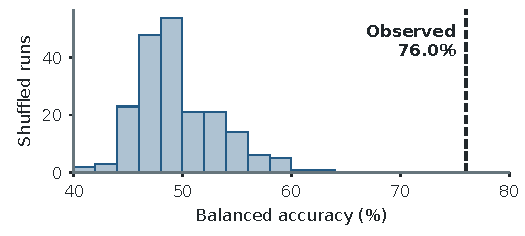
\includegraphics[width=\columnwidth]{figures/permutation-accuracy.pdf}
\caption{Balanced accuracy of the eight-question procedure with the observed labels (dashed line) and across 199 shuffled-label evaluations. Each value averages five cross-validation repetitions.}
\label{fig:permutation-accuracy}
\end{figure}

Table~\ref{tab:warning-intervals} gives conditional intervals for the forest and the paired differences between the forest and workload-only logistic regression. The interval calculation resampled students with the fitted predictions held fixed. All three paired intervals included zero. Across the five cross-validation repetitions, the forest's recall ranged from 82.4\% to 94.1\%, and its false-warning count ranged from 24 to 30.

\begin{table}[t]
\caption{Conditional 95\% Intervals for Warning Performance}
\label{tab:warning-intervals}
\centering
\footnotesize
\begin{tabular}{@{}lrr@{}}
\hline
Metric & \shortstack[b]{Forest\\(\%)} & \shortstack[b]{Forest minus workload\\(percentage points)} \\
\hline
Recall & 70.6 to 100.0 & \(-20.0\) to \(2.4\) \\
Precision & 27.9 to 42.7 & \(-7.3\) to \(3.1\) \\
Balanced accuracy & 66.4 to 83.8 & \(-11.1\) to \(2.3\) \\
\hline
\end{tabular}
\end{table}

\subsection{Earlier Warning Comparisons and Synthetic Check}

Earlier experiment records show the trade-off between detecting High students and issuing false warnings. Under \(F_2\) tuning, the 23-input support vector classifier averaged 13.0 High detections and 19.4 false warnings. The forest fitted with inputs selected by Boruta~\cite{kursa2010boruta} averaged 12.4 High detections and 22.2 false warnings. Both procedures detected fewer High students than the selected forest.

In an earlier comparison using the same eight inputs, TabPFN-2~\cite{hollmann2025tabpfn} had higher average precision (0.616) than the selected forest. The TabPFN-2 rule selected using \(F_2\) averaged 13.8 High detections and 24.2 false warnings. The rule tuned to favor recall averaged 15.2 High detections and 44.0 false warnings.

The synthetic check used 970 profiles generated from survey responses already used to fit the model. The model fitted on all 97 students flagged 159 of the 170 profiles assigned a High label (93.5\%). This rate measures agreement with the High labels inherited from the source responses.

\subsection{Discussion}

The measured reduction in ridge regression error applies to the three GenAI questions together. AI dependence had the strongest individual association with the burnout score among those three questions. Plensamai reported a positive association in the same direction among Thai undergraduates using a different burnout measure~\cite{plensamai2026burnout}. An additional matched comparison that adds AI dependence alone would be needed to estimate its individual contribution to prediction.

At the chosen warning thresholds, workload-only logistic regression detected more High cases at the same average false-warning count as the random forest. The warning comparison varied both the classifier and the inputs, so these results compare the two procedures as a whole.

About two of every three warnings from the selected forest went to students with a burnout score below the study cutoff. Of the 80 Below-high students, 39 received at least one false warning across the five repetitions, and 27 received a false warning in at least three repetitions.

The survey measured GenAI habits, study conditions, and symptoms at one time. The order of events therefore remains unresolved. The convenience sample contained 17 High cases, and several model and input choices followed earlier analyses of the same students. The permutation test applies to the selected forest procedure, and the paired intervals apply to its comparison with workload-only logistic regression. Estimating warning performance in a new cohort requires fixing each procedure in advance and evaluating it on independently recruited students with measured BAT-S outcomes.
